%!TEX root = predictability.tex

\subsection{Experiment Setup}
The instances we used for running MySQL and the one we used to send 
transactions to MySQL have the same configuration as those described in
section 4.1. Unless explicitly mentioned, the storage devices of these
instances are traditional magnetic disks. There are three different types of
workloads we use in our experiments. The first one is the original TPC-C
benchmark, which is an OLTP benchmark with 5 different types of transactions.
Each type of transaction could have different number of queries for each
transaction. The second one is TPC-C benchmark with only New Order 
transactions(TPC-C New Order). The number of queries in a New Order
transaction is $5 + 4x$ in which $x$ is a random number ranging from 5 to 15.
The third one is TPC-C benchmark with New Order transactions that consist of
exactly 45($x$ = 10 in the formula above) queries(TPC-C New Order Fixed).

\subsection{Combing Every Possible Method}
In this section, we show the best result we can have by combining every
possible method we have for reducing the variance of transaction latency.
We create a ramdisk, and install MySQL to that ramdisk. The \texttt{datadir}
of MySQL is also set to a directory on the ramdisk. We set the value of
\texttt{innodb\_flush\_log\_at\_trx\_commit} to 2 and the value of
\texttt{innodb\_buffer\_pool\_size} to 1024M, and we implement the techniques
we describe in section 5 in MySQL. Figure \ref{fig:all-mean} and
\ref{fig:all-throughput} show the improvement in performance under the original
TPC-C benchmark, TPC-C New Order and TPC-C New Order Fixed, respectively.
Figure \ref{fig:all-std-mean} and \ref{fig:all-99-mean} show the improvement in
variance of transaction latency under these three types of workloads. In all
cases, the combined method outperform the original MySQL both in performance
and variance in transaction latency. Also, the variance of latency decrease as
the workload changes from the original TPC-C to TPC-C New Order to TPC-C New
Order Fixed. This makes sense because the discrepancy of transactions in these
three types of workloads decreases as the type of transaction is fixed, and the
number of queries in each transaction is fixed. Obviously, the variance of
transactions in the workloads also have an impact on the variance of latency,
which is quite natural.

\begin{figure*}
    \centering
    \begin{subfigure}[t]{0.24\textwidth}
        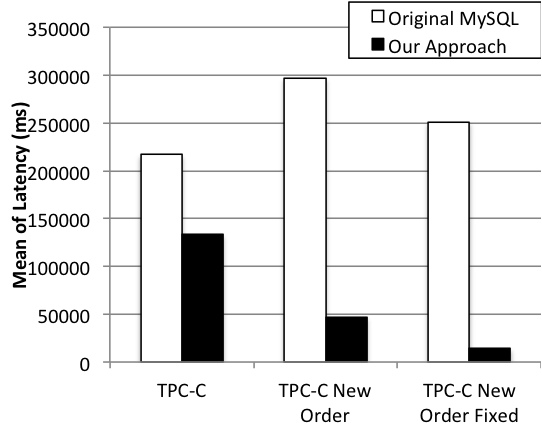
\includegraphics[width=\textwidth]{plots/all/latency}
        \caption{Average Latency}
        \label{fig:all-mean}
    \end{subfigure}
    \begin{subfigure}[t]{0.24\textwidth}
        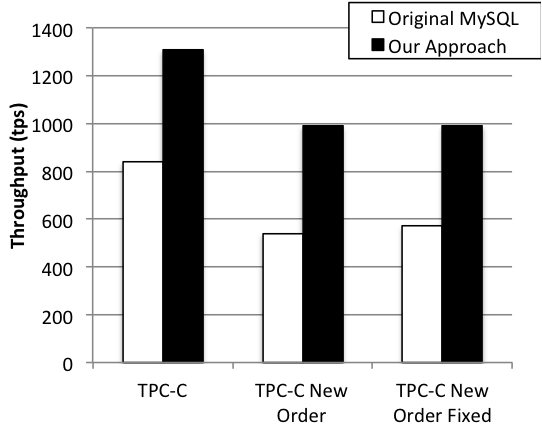
\includegraphics[width=\textwidth]{plots/all/throughput}
        \caption{Throughput}
        \label{fig:all-throughput}
    \end{subfigure}
    \begin{subfigure}[t]{0.24\textwidth}
        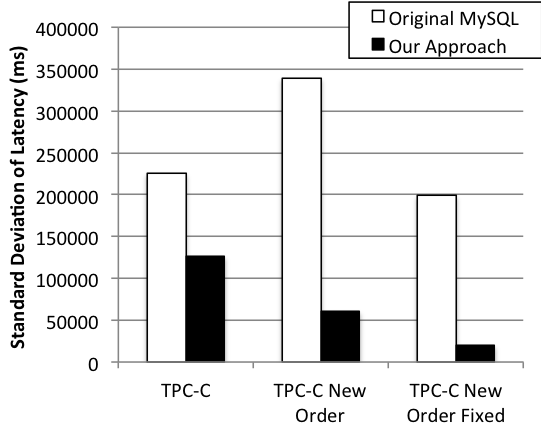
\includegraphics[width=\textwidth]{plots/all/std}
        \caption{Standard Deviation / Mean}
        \label{fig:all-std-mean}
    \end{subfigure}
    \begin{subfigure}[t]{0.24\textwidth}
        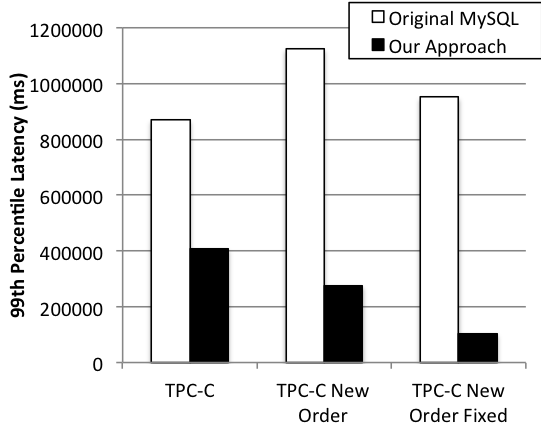
\includegraphics[width=\textwidth]{plots/all/99}
        \caption{99th Percentile / Mean}
        \label{fig:all-99-mean}
    \end{subfigure}
    \caption{Effect of All Methods Combined}
    \label{fig:all-combined}
\end{figure*}

\subsection{Evaluation of Fixes for \texttt{buf\_pool\_mutex\_enter}}
In this section we evaluate the effects of the two techniques presented in
section 5 on the variance of latency. We first implement these two techniques
in MySQL separately and run experiments on them using all three different
types of workloads. We compare the results of applying these two methods to
the original MySQL, respectively. The finer-grained locking mechanism is
referred to as ``FG'' in figure \ref{fig:fixes} and the spin lock with timeout
technique is referred to as ``SL'' in it. Both of them show improvement in
variance of latency without negative impact on the performance. Actually, they
improves not only variance, but also performance, especially the average
latency. The throughput of MySQL also receives a small increase. This is
because these two methods both reduce contention among different functions(one
by using finer-grained lock and the other by giving up lock requisition when
times out), thus reducing the time the related functions spend on waiting for
other functions. We then apply both of these two methods on MySQL, and a
greater reduction in variance than any of these two methods alone is shown.
Both standard deviation and 99th percentile reduce by more than 40\% with the
original TPC-C workload. For TPC-C New Order and TPC-C New Order Fixed, the
reductions are more than 50\%.

\begin{figure*}
    \centering
    \begin{subfigure}[t]{0.24\textwidth}
        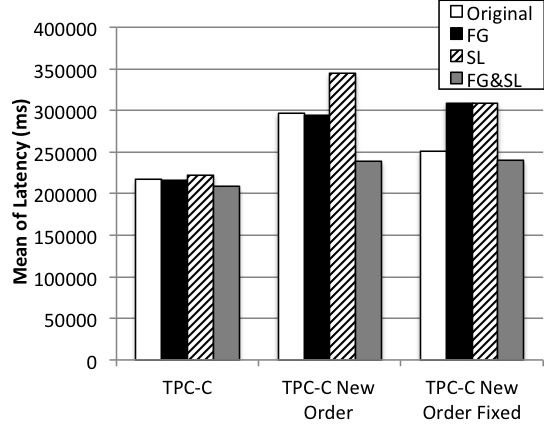
\includegraphics[width=\textwidth]{plots/ours/latency}
        \caption{Average Latency}
        \label{fig:fix-mean}
    \end{subfigure}
    \begin{subfigure}[t]{0.24\textwidth}
        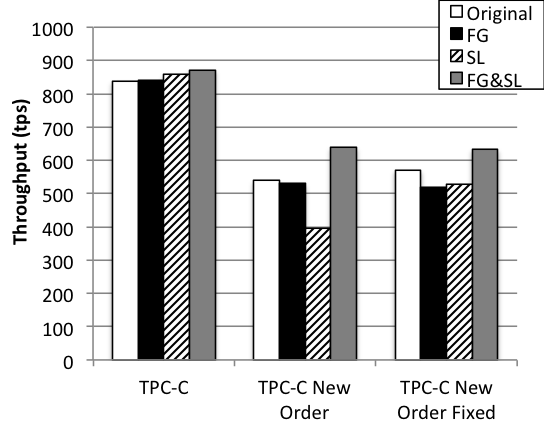
\includegraphics[width=\textwidth]{plots/ours/throughput}
        \caption{Throughput}
        \label{fig:fix-throughput}
    \end{subfigure}
    \begin{subfigure}[t]{0.24\textwidth}
        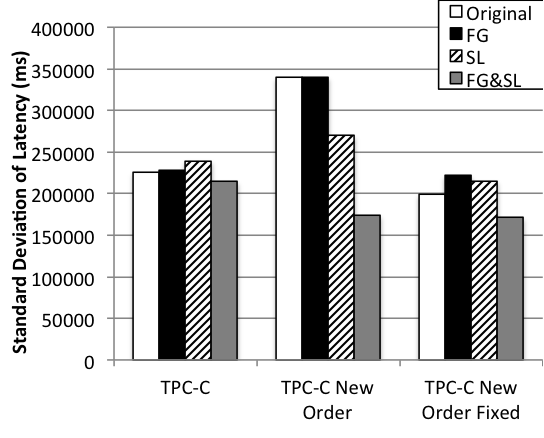
\includegraphics[width=\textwidth]{plots/ours/std}
        \caption{Standard Deviation}
        \label{fig:fix-std-mean}
    \end{subfigure}
    \begin{subfigure}[t]{0.24\textwidth}
        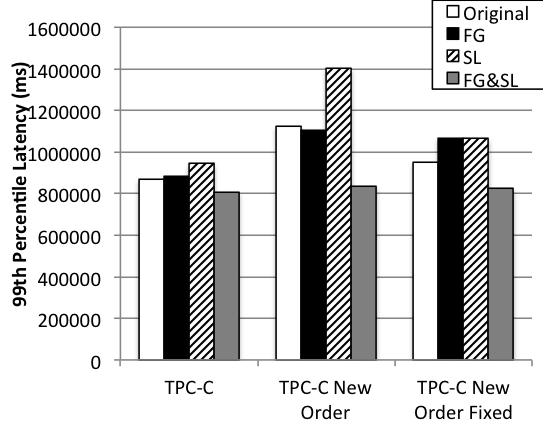
\includegraphics[width=\textwidth]{plots/ours/99}
        \caption{99th Percentile}
        \label{fig:fix-99-mean}
    \end{subfigure}
    \caption{Effect of Fixes for \texttt{buf\_pool\_mutex\_enter}}
    \label{fig:fixes}
\end{figure*}

\subsection{Using Faster Storage}
In this section we evaluate the effect of using faster storage devices on
the variance of transaction latency. We run MySQL on three different instances,
one with traditional HDD, one with SSD and one with a magnetic disk and a
ramdisk, where MySQL is installed and all the data are stored. A ramdisk is
simply a block of memory treated as a normal disk device by applications. It's
a way of simulating a super-fast disk using memory, and the data would still
be lost when powered off just like normal memory. As can be seen from figure
\ref{fig:storage}, there's huge improvement in performance when changing from
HDD to SSD and ramdisk. Also, along with that, the standard deviation and 99th
percentile of latency also decrease.

\begin{figure*}
    \centering
    \begin{subfigure}[t]{0.24\textwidth}
        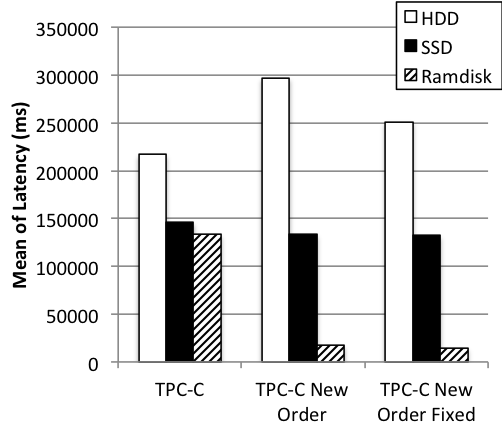
\includegraphics[width=\textwidth]{plots/storage/latency}
        \caption{Average Latency}
        \label{fig:storage-mean}
    \end{subfigure}
    \begin{subfigure}[t]{0.24\textwidth}
        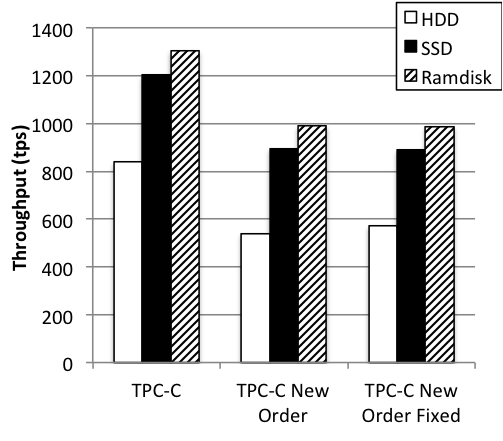
\includegraphics[width=\textwidth]{plots/storage/throughput}
        \caption{Throughput}
        \label{fig:storage-throughput}
    \end{subfigure}
    \begin{subfigure}[t]{0.24\textwidth}
        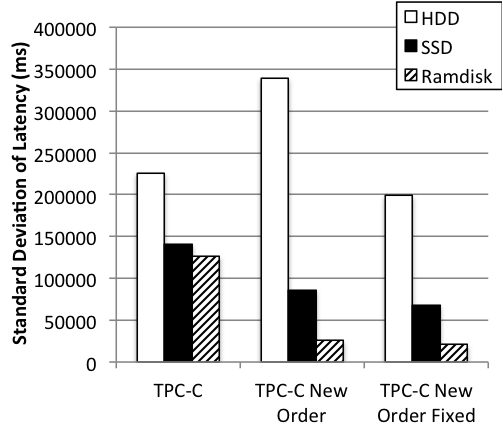
\includegraphics[width=\textwidth]{plots/storage/std}
        \caption{Standard Deviation/Mean}
        \label{fig:storage-std-mean}
    \end{subfigure}
    \begin{subfigure}[t]{0.24\textwidth}
        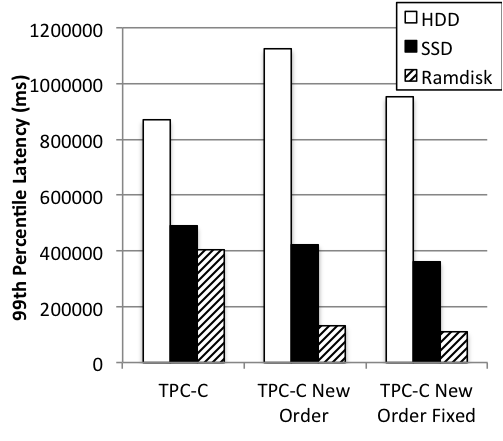
\includegraphics[width=\textwidth]{plots/storage/99}
        \caption{99th Percentile/Mean}
        \label{fig:storage-99-mean}
    \end{subfigure}
\caption{Effect of Faster Storage Device}
\label{fig:storage}
\end{figure*}

\subsection{Variance-away Tuning}
In this section, we evaluate the effects different parameters of MySQL have
on the variance of latency. We pick two parameters that we consider as
closely related to the variance of latency. The first one is the size of the
buffer pool. We increase the size of the buffer pool from 1GiB(default value)
to 5GiB. Obviously increasing the buffer pool size keeps more data in memory,
thus effectively reducing the number of buffer page replacements, the number of
I/O operations and also contention within the buffer pool. As we can see from
the results shown in figure \ref{fig:buffer_pool_size}, the larger the size of
buffer pool, the lower the average latency, standard deviation and 99th
percentile. Setting the size of the buffer pool to as large as possible is
recommended both for better performance and for higher predictability.

The second parameter that we choose and run experiments on is
\texttt{innodb\_flush\_log\_at\_trx\_commit}. This parameter affects MySQL's
strategy for flushing redo logs to disk when transactions are committed. The
default value of this option is 1, which means that logs are flushed to disk
whenever a transaction is committed. When this value is set to 0, MySQL write
the redo logs to the log files and flush the data to disk once per second, but
nothing is done when transactions commit. When this value is set to 2, redo
logs are written to the log file at transaction commit, but flush operations
are done once per second. Although this parameter is only directly related to
redo logs, changing it to 0 or 2 effectively reduces the number of I/O
operations for redo logs by grouping multiple operations into one. Experiment
result in figure \ref{fig:log_flush} shows that setting it to 0, namely
grouping multiple write operations and flush operations together, is generally
better than 2, which is to group only flush operations on performance and
variance of latency.

However, setting this option to 0 or 2 is risky. If the option is set to 0,
which means that log data is written to file and flushed to disk once per
second, and MySQL crashes, all the transactions in the last second will be gone
and cannot be recovered. On the other hand, when this option is set to 2,
namely only write the logs to the file, the transactions in the last second
will be lost when the operating system crashes(log data is safe even if MySQL
crashes with this option). Therefore, this option is only suitable for
applications that do not require high data consistency, such as forums, blogs,
but not acceptable for applications like bank systems.

\begin{figure*}
    \centering
    \begin{subfigure}[t]{0.24\textwidth}
        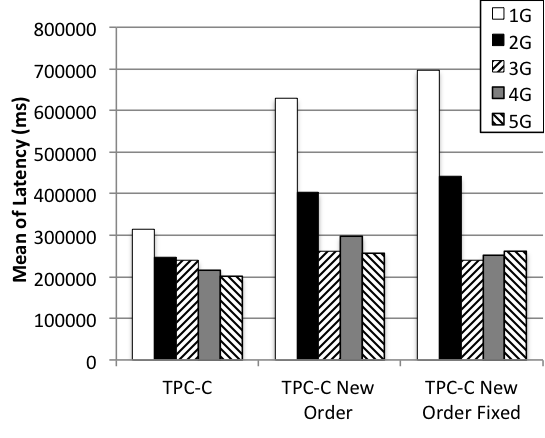
\includegraphics[width=\textwidth]{plots/buffer_pool_size/latency}
        \caption{Average Latency}
        \label{fig:buf-size-mean}
    \end{subfigure}
    \begin{subfigure}[t]{0.24\textwidth}
        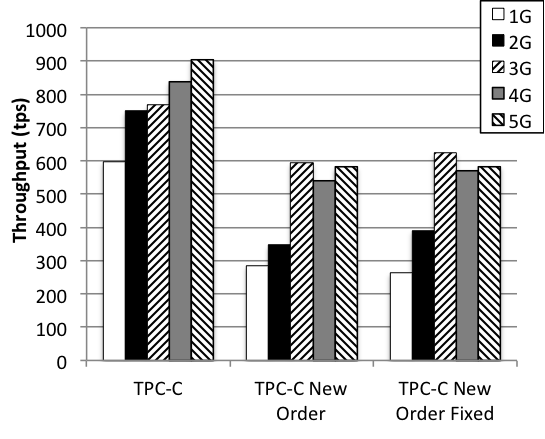
\includegraphics[width=\textwidth]{plots/buffer_pool_size/throughput}
        \caption{Throughput}
        \label{fig:buf-size-throughput}
    \end{subfigure}
    \begin{subfigure}[t]{0.24\textwidth}
        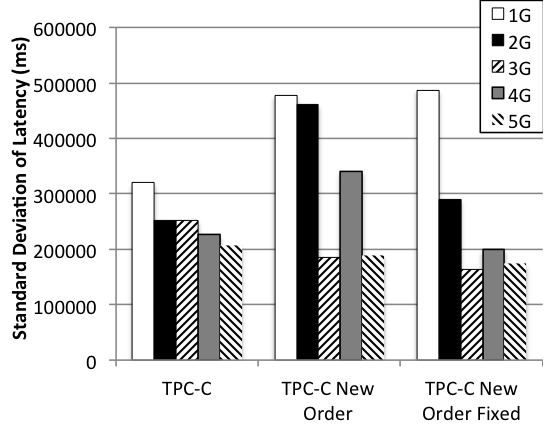
\includegraphics[width=\textwidth]{plots/buffer_pool_size/std}
        \caption{Standard Deviation}
        \label{fig:buf-size-std-mean}
    \end{subfigure}
    \begin{subfigure}[t]{0.24\textwidth}
        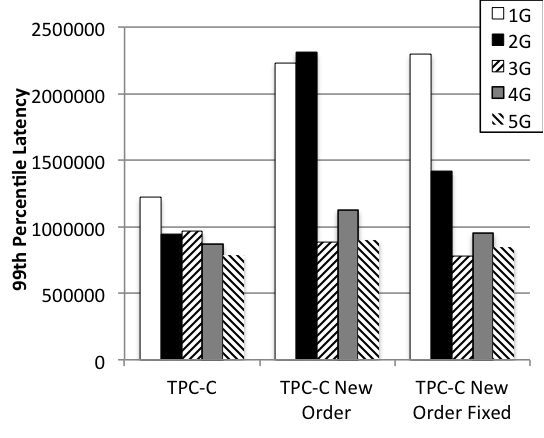
\includegraphics[width=\textwidth]{plots/buffer_pool_size/99}
        \caption{99th Percentile}
        \label{fig:buf-size-99-mean}
    \end{subfigure}
\caption{Effect of Buffer Pool Size}
\label{fig:buffer_pool_size}
\end{figure*}

\begin{figure*}
    \centering
    \begin{subfigure}[t]{0.24\textwidth}
        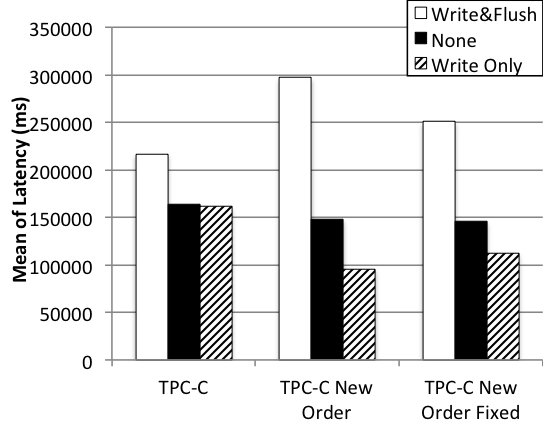
\includegraphics[width=\textwidth]{plots/log_flush/latency}
        \caption{Average Latency}
        \label{fig:commit-mean}
    \end{subfigure}
    \begin{subfigure}[t]{0.24\textwidth}
        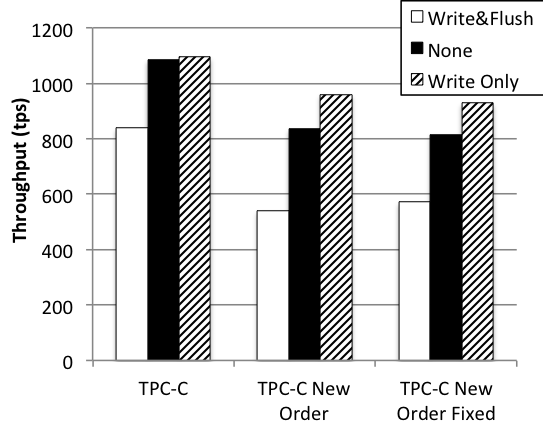
\includegraphics[width=\textwidth]{plots/log_flush/throughput}
        \caption{Throughput}
        \label{fig:commit-throughput}
    \end{subfigure}
    \begin{subfigure}[t]{0.24\textwidth}
        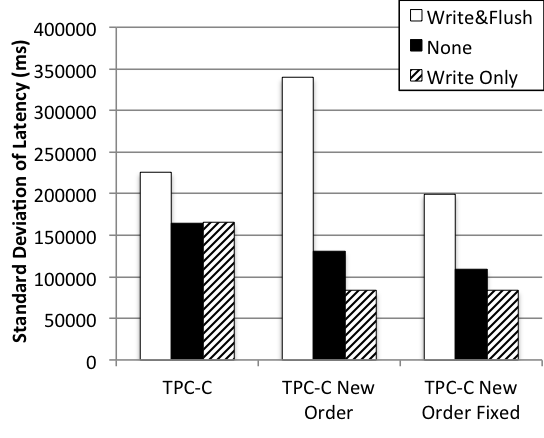
\includegraphics[width=\textwidth]{plots/log_flush/std}
        \caption{Standard Deviation}
        \label{fig:commit-std-mean}
    \end{subfigure}
    \begin{subfigure}[t]{0.24\textwidth}
        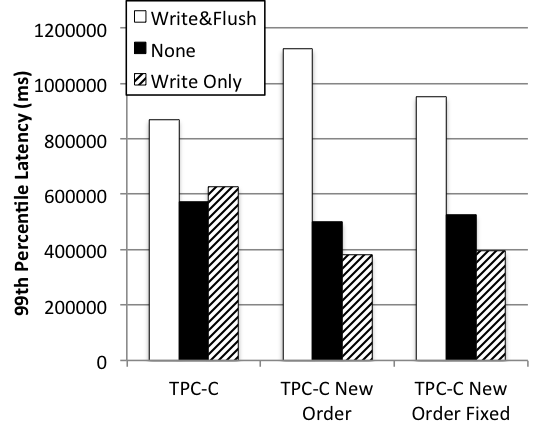
\includegraphics[width=\textwidth]{plots/log_flush/99}
        \caption{99th Percentile}
        \label{fig:commit-99-mean}
    \end{subfigure}
\caption{Effect of Log Flush Policy}
\label{fig:log_flush}
\end{figure*}

\subsection{Evaluation of VProfiler}
In this section, we evaluate the performance overhead VProfiler introduces
into MySQL when it monitors the execution time of a \textit{parent function}
and its \textit{child functions} to break down the \textit{parent function's}
variance, and its efficiency in finding the main sources of variance in MySQL.

\subsubsection{VProfiler vs. DTrace}
VProfiler breaks down the variance of a \textit{parent function} into the
variances and covariances of its \textit{child functions} by monitoring the
execution time of the \textit{parent functions} and every \textit{child
function}. This introduces overhead to the system. In this section, we change
the number of \textit{child functions} VProfile needs to monitor and measure
its performance overhead in terms of reduction average latency and throughput.

As a comparison, we also evaluate the performance overhead of DTrace. Due to
its incomplete support on Linux, we had to run a virtual machine on VirtualBox
with 10 Intel Xeon E5-2450 2.10GHz virtual CPUs and 15GiB of memory and
run Solaris 11 on it.

\begin{figure}
    \centering
    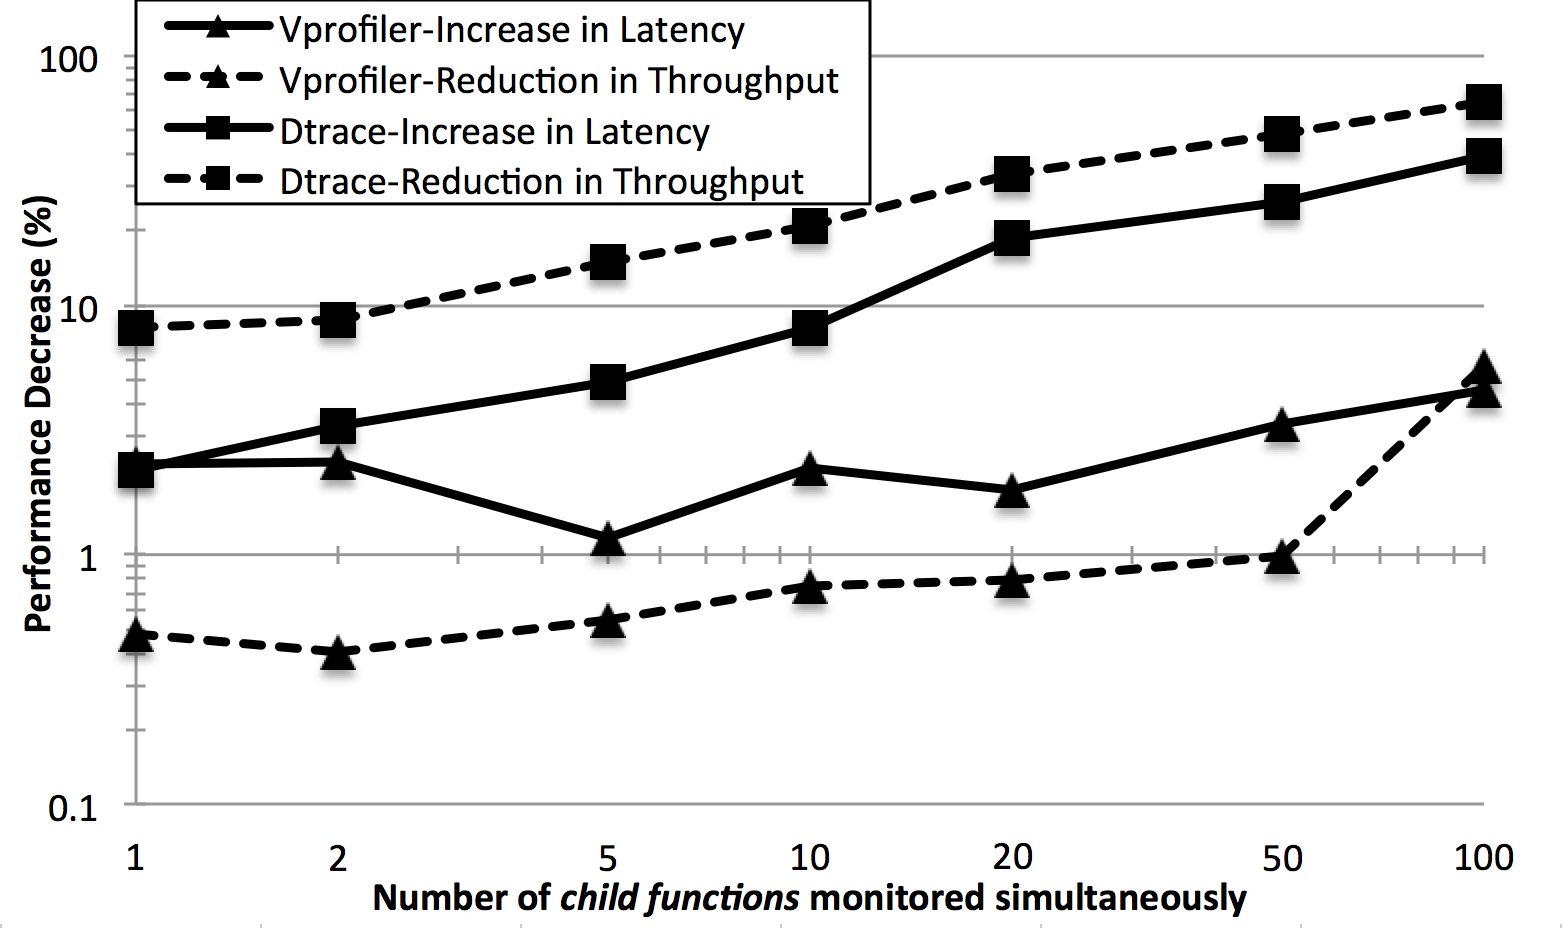
\includegraphics[scale=0.3]{plots/overhead}
\caption{Profiler overhead: VProfiler vs. DTrace}
\label{fig:overhead}
\end{figure}

In this experiment, we change the number of \textit{child functions} to trace
from 1 to 100. Figure \ref{fig:overhead} shows the experiment results. We can
see that the overhead of DTrace is a lot higher than VProfiler. The overhead of
DTrace in terms of reduction in latency and throughput grows rapidly as the
number of child functions it traces simultaneously increase, while the overhead
of VProfiler stays below 6\%, because the monitoring technique VProfiler uses
is pretty lightweight.

\subsubsection{VProfiler vs. Naïve Profiler}
In this section, we compare VProfiler to a na\"{\i}ve profiler, which is very
similar to VProfiler but breaks down every factor when possible instead of only
a few important ones. We use this profiler on MySQL and evaluate the number of
experiments this profiler has to run to find out the main sources of variance
with different numbers of functions to monitor simultaneously in each 
experiment.

\begin{figure}
    \centering
    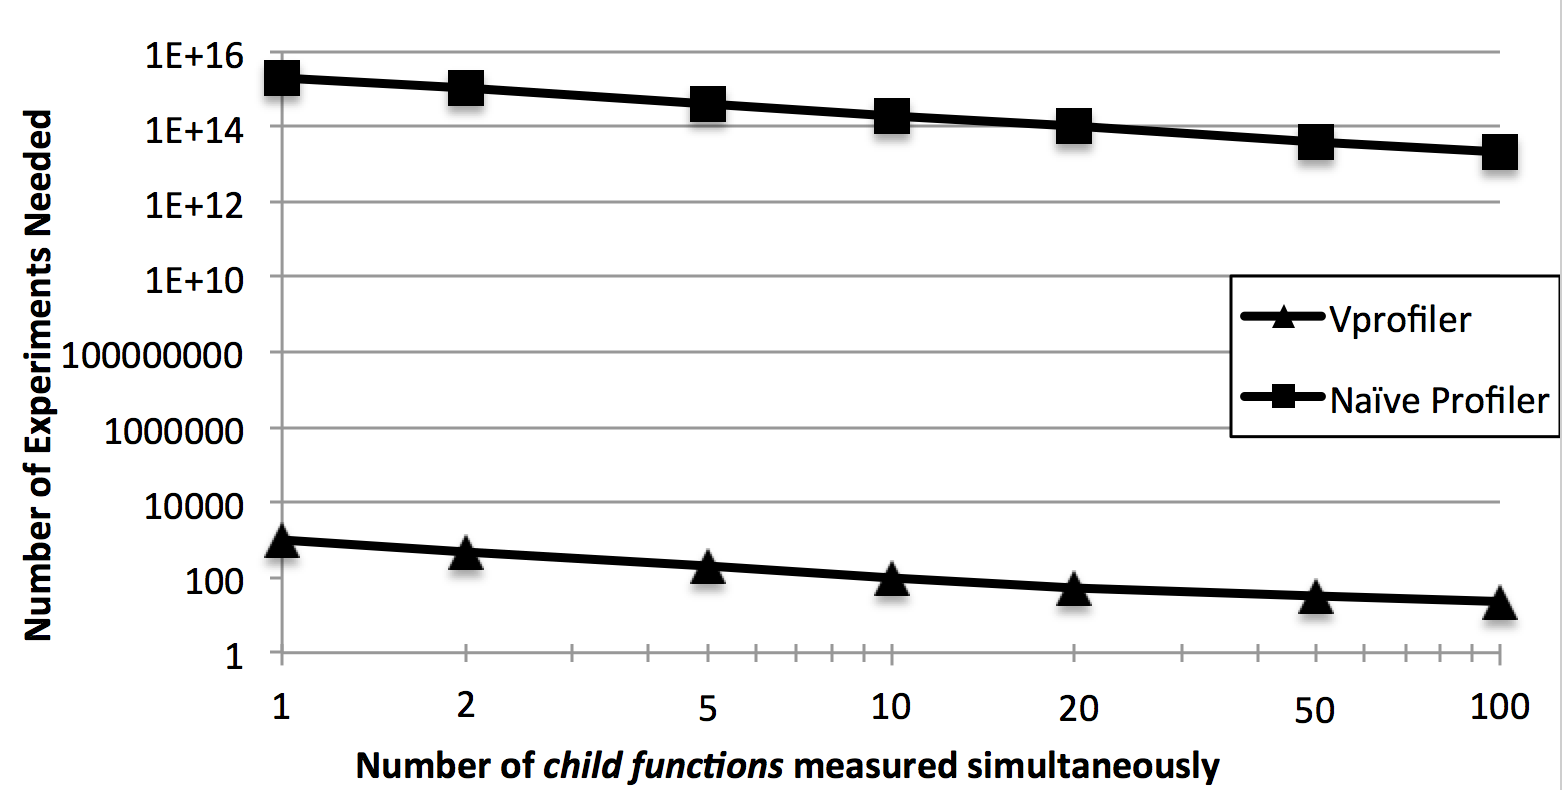
\includegraphics[scale=0.3]{plots/experiments}
\caption{Number of experiments needed for the profiler to find out the main sources of variance}
\label{fig:experiments}
\end{figure}

There are totally $2 \times 10^{15}$ nodes in the call graph(one function 
called in multiple places are regarded as different nodes in the graph),
$4.5 \times 10^{14}$ of which being leaves. Since the na\"{\i}ve profiler has
to break down every non-leaf nodes, the number of experiments needed is
extremely large. The selection strategy of VProfiler greatly reduces the number
of experiment it has to run to locate the main sources of variance.
